% =====================================================================
% Chương 03 — Lớp Xử lý (Processing)
% Phân tích: tools/test_mqtt_coreiot.py, supersonic_rule_chain.json,
%            tools/guard/check_rulechain_thresholds.py
% =====================================================================

\chapter{Lớp Xử lý (Processing)}
\label{ch:processing}

Lớp Xử lý nằm giữa Lớp Cảm biến (nơi dữ liệu thô được lọc) và Lớp Ứng dụng
(nơi hiển thị cảnh báo).  Trên \textbf{sensor-node}, bản sao knn-filtered
\code{sharedStateGetNearest()} được truyền thẳng sang ESP-NOW.  Trên
\textbf{đường phụ MQTT/CoreIoT}, dữ liệu \code{d1..d6 + nearest\_cm} đi lên
broker, nơi \textbf{rule-chain} xử lý thành \code{warning\_status} rồi đẩy xuống
\code{waveshare-screen}.

\section{Tool kiểm thử MQTT (R1/R3/R11)}

\begin{center}
\begin{longtable}{@{}p{4.2cm}p{3.8cm}p{6.0cm}@{}}
  \toprule
  \textbf{Thuộc tính} & \textbf{Giá trị} & \textbf{Ghi chú} \\
  \midrule
  \endhead
  File & \code{tools/test\_mqtt\_coreiot.py} & 217 dòng, Python 3.12+ \\
  Broker & \code{app.coreiot.io:1883} & ThingsBoard CE (CoreIoT) \\
  Topic & \code{v1/devices/me/telemetry} & \code{username = access\_token} \\
  Payload keys & \code{d1..d6, nearest\_cm,} & mirror firmware/SIM/I \\
  & \code{has\_nearest, warning\_status} & (thresholds.h $\rightarrow$ classify) \\
  Token nguồn & \code{config/keys.json} & R1: \textbf{không} hardcode \\
  Dry-run & \code{--dry-run} & in payload, \textbf{không} kết nối MQTT \\
  \bottomrule
\end{longtable}
\end{center}

\textbf{Hàm chính:}
\begin{itemize}
\item \code{classify(distance)} (\code{test\_mqtt\_coreiot.py:55}): trả
  \code{"DANGER"} nếu $\leq 30$, \code{"CAUTION"} nếu $\leq 100$, ngược lại
  \code{"NORMAL"}.
\item \code{build\_payload(distance, seq)} (\code{test\_mqtt\_coreiot.py:64}):
  tạo dict với \code{d1..d6 = distance}, \code{nearest\_cm = distance},
  \code{has\_nearest = True}, \code{warning\_status = classify(...)},
  \code{vehicle\_detected}, \code{timestamp} (epoch ms), \code{seq} (tuỳ chọn).
\item \code{resolve\_token(args, cfg)} (\code{test\_mqtt\_coreiot.py:78}):
  ưu tiên \code{--token} $>$ env \code{COREIOT\_TOKEN} $>$
  \code{config/keys.json.SENSOR\_NODE\_DEVICE\_TOKEN}.
\item \code{run\_publisher(args)} (\code{test\_mqtt\_coreiot.py:133}): kết nối
  MQTT (\code{paho.mqtt}), gửi \code{json.dumps(payload)}, hỗ trợ
  \code{--loop --interval}.
\end{itemize}

\section{Sơ đồ Rule-Chain (7 nút)}
\label{sec:rulechain-graph}

\begin{center}
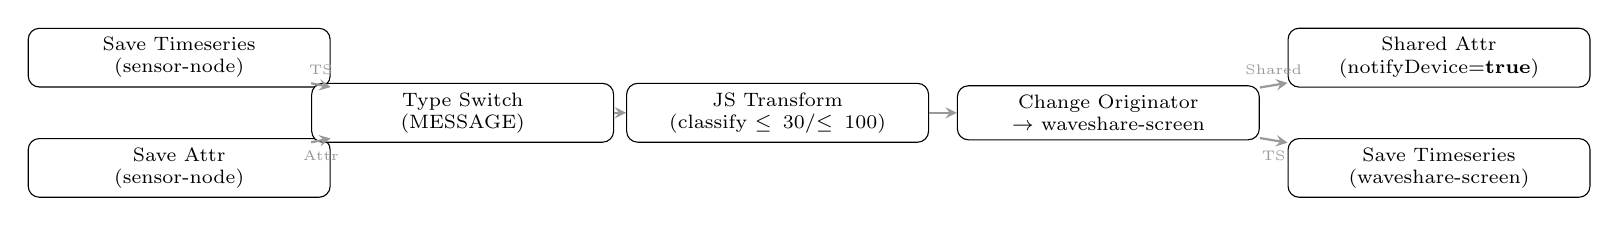
\begin{tikzpicture}[
  node distance=1.4cm and 1.6cm,
  box/.style={draw, rounded corners, font=\scriptsize, align=center,
               text width=3.6cm, fill=white},
  arrow/.style={-stealth, thick, gray!80},
]
% Nút 0-1: đỉnh trái
\node[box] (saveTS0)  {Save Timeseries\\(sensor-node)};
\node[box, below of=saveTS0] (saveA1) {Save Attr\\(sensor-node)};
% Nút 2: trung tâm trái
\node[box, right of=saveTS0, xshift=2.2cm, yshift=-0.7cm]
  (sw2) {Type Switch\\(MESSAGE)};
% Nút 3: trung tâm phải
\node[box, right of=sw2, xshift=2.6cm] (js3)
  {JS Transform\\(classify $\leq 30$/$\leq 100$)};
% Nút 4: phải
\node[box, right of=js3, xshift=2.8cm] (ori4)
  {Change Originator\\$\rightarrow$ waveshare-screen};
% Nút 5-6: đỉnh phải
\node[box, right of=ori4, xshift=2.8cm, yshift=0.7cm]
  (shared5) {Shared Attr\\(notifyDevice=\textbf{true})};
\node[box, below of=shared5] (saveTS6)
  {Save Timeseries\\(waveshare-screen)};

% Liên kết
\draw[arrow] (sw2) -- node[above,font=\tiny]{TS}(saveTS0);
\draw[arrow] (sw2) -- node[below,font=\tiny]{Attr}(saveA1);
\draw[arrow] (sw2) -- (js3);
\draw[arrow] (js3) -- (ori4);
\draw[arrow] (ori4) -- node[above,font=\tiny]{Shared}(shared5);
\draw[arrow] (ori4) -- node[below,font=\tiny]{TS}(saveTS6);
\end{tikzpicture}
\end{center}

\textbf{Luồng dữ liệu:} \code{sensor-node} gửi telemetry $\rightarrow$
\textbf{TypeSwitch} (\#2) $\rightarrow$ ba nhánh: (1) lưu TS sensor-node (\#0),
(2) lưu Attr sensor-node (\#1), (3) \textbf{JS Transform} (\#3) $\rightarrow$
\textbf{ChangeOriginator} (\#4) $\rightarrow$ hai nhánh: shared Attr với
\textbf{notifyDevice=true} (\#5) để \code{waveshare-screen} nhận qua MQTT, lưu
TS waveshare-screen (\#6).

\section{JS Transform — Phân loại khoảng cách}

Script JavaScript trong nút \#3 (\code{supersonic\_rule\_chain.json:79--81})
thực hiện phân loại \textbf{giống hệt} firmware:
\begin{enumerate}
\item Lấy \code{nearest\_cm} nếu \code{has\_nearest == true};
  nếu không, tìm min trong \code{[d1..d6]}.
\item Phân loại: \code{distance $\leq$ 30.0} $\rightarrow$ \textbf{DANGER};
  $\leq 100.0$ $\rightarrow$ \textbf{CAUTION}; else \textbf{NORMAL}.
\item Tạo \code{warning\_status}, \code{vehicle\_detected}, \code{relay},
  \code{buzzer}, \code{nearest\_cm}, \code{source\_device}.
\item Trả về \code{msgType: "POST\_ATTRIBUTES\_REQUEST"} — quy ước
  ThingsBoard ghi \textbf{shared attributes}, không phải timeseries.
\end{enumerate}

\noindent\textbf{Giá trị hằng số trong JS (R3):} \code{30.0} và \code{100.0}
hardcoded trong script, khớp \code{thresholds.h} \code{DANGER\_CM = 30} /
\code{CAUTION\_CM = 100}.  Script \code{check\_rulechain\_thresholds.py}
kiểm tra sự khớp này tại mỗi lần build (xem §\ref{sec:threshold-check}).

\section{Validate Thresholds (R3/R11)}
\label{sec:threshold-check}

\begin{center}
\begin{longtable}{@{}p{4.5cm}p{3.5cm}p{5.5cm}@{}}
  \toprule
  \textbf{Tool} & \textbf{Thực thi} & \textbf{Cơ chế} \\
  \midrule
  \endhead
  \code{check\_rulechain\_thresholds.py} & \code{CI + local} & Tải
  \code{thresholds.h} (grep \code{CAUTION\_CM}, \code{DANGER\_CM}) +
  \code{rule\_chain.json} (grep \code{30.0}, \code{100.0}) \\
  Exit code & \code{0 = khớp} & Nếu bất kỳ ngưỡng nào lệch: exit 1 + in
  giá trị lệch \\
  CI gate & \code{ci.yml} & Chạy \code{python3 tools/guard/
  check\_rulechain\_thresholds.py}; fail $\rightarrow$ CI đỏ \\
  \bottomrule
\end{longtable}
\end{center}

\textbf{Trích yếu kiểm tra (R3):} mọi ngưỡng zone \textbf{chỉ có một nguồn}
tại \code{firmware/shared/thresholds.h}.  Rule-chain JSON là
\textbf{snapshot} có thể đối chiếu — khi đổi ngưỡng, phải sửa
\code{thresholds.h} trước, rule-chain được import lại trên ThingsBoard console
(Cổng B0b), và \code{check\_rulechain\_thresholds.py} xác nhận khớp.

\section{Tóm tắt luồng xử lý}
\label{sec:processing-summary}

\begin{center}
\begin{tabular}{@{}lll@{}}
  \toprule
  \textbf{Điểm bắt đầu} & \textbf{Điểm kết thúc} & \textbf{Kênh} \\
  \midrule
  \code{sharedStateGetNearest()} &
    \code{espnow\_send(...)} & ESP-NOW (chính) \\
  \code{coreiotTask:} \code{json\_dump\_d1..d6} &
    Rule-chain $\rightarrow$ screen & MQTT (phụ) \\
  Rule-chain JS Transform &
    \code{Shared Attr: warning\_status} &
    MQTT notifyDevice \\
  \bottomrule
\end{tabular}
\end{center}
